\chapter{Introduzione}
\label{chap:introduzione}

\section{Contesto e limiti delle onde elettromagnetiche}
Le reti di sensori in ambienti sotterranei pongono sfide peculiari alla comunicazione wireless. 
La propagazione delle \emph{onde elettromagnetiche} nel sottosuolo soffre di attenuazioni elevate dovute alla 
permittività, alla conducibilità del terreno e all'umidità, con conseguente riduzione drastica della portata e 
dell'affidabilità dei link radio \citep[pp.~24--59]{Lee2000_RadioWavePropagationTunnels}. 

Alcune soluzioni proposte in letteratura includono l'uso di frequenze super-high ed ultra-high (SHF, UHF) con l'obiettivo 
di implementare sistemi di tracking e monitoraggio in miniere di carbone, gallerie o condotti \citep{jacksha2016}.
Tuttavia, queste frequenze a causa della loro natura fisica sono soggette a forti perdite di segnale e riflessioni multipath,
limitando la copertura a range dai 10 ai 33 metri in condizioni ottimali con l'ausilio di antenne direzionali con un altezza 
pari a 1.2 metri l'una; questa tecnologia inoltre mostra tutta la sua vulnerabilità in presenza di curve strette (90°) o ostacoli.

\begin{figure}[H]
    \centering
    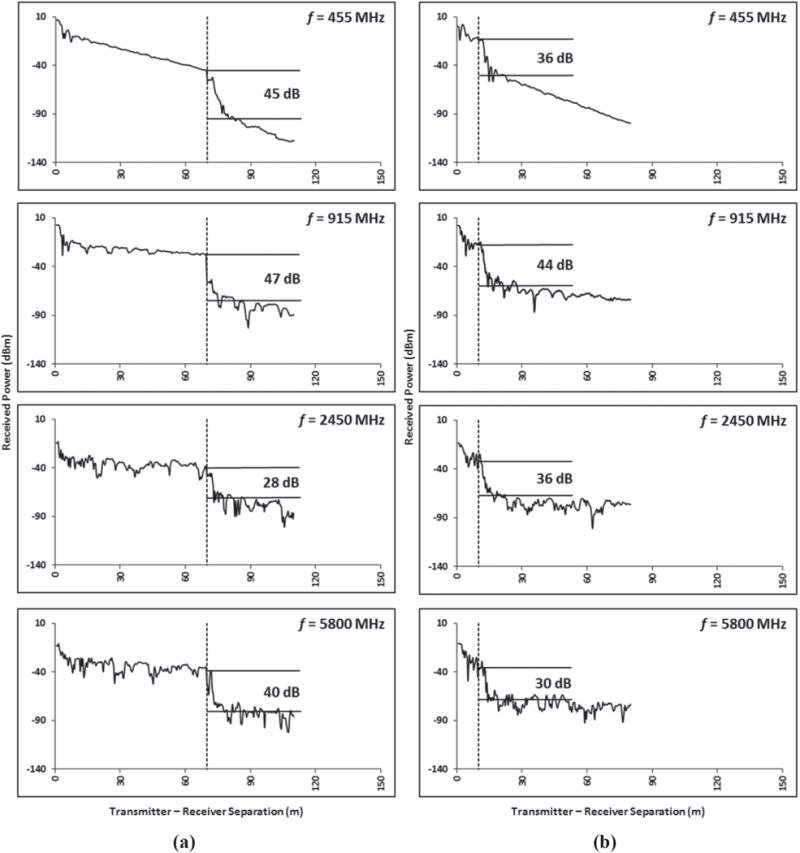
\includegraphics[width=0.35\textwidth]{immagini/corner_loss_em.jpg}
    \caption{Corner Loss \textasciitilde 30 dB in un condotto con angolo di 90° per radio frequenze HF/SHF \citep{jacksha2016}.}
    \label{fig:esempio}
\end{figure}

\section{Motivazione dell’approccio acustico}
Da questa problematica nasce la presente tesi, che si pone l’obiettivo di progettare e validare un 
\textbf{protocollo di comunicazione acustica} per reti \textbf{master--slave} in ambienti sotterranei, che dovrà essere: \textbf{efficiente, robusta ed economica}. 

L’idea è sfruttare la \emph{propagazione del suono nell’aria} presente in cavità, condotti o tunnel, trattando l’aria 
come un canale guida all'interno degli spazi confinati, e più in generale impiegare l’onda acustica come 
mezzo portante laddove il canale elettromagnetico è troppo penalizzato. 

\section{Richiami teorici sulla propagazione acustica}
In effetti, l’aria può essere modellata come un fluido compressibile: le variazioni locali di pressione e densità generate da una sorgente si propagano come onde longitudinali, 
la cui dinamica è descritta dall’equazione delle onde acustiche. 
La velocità di propagazione, che in condizioni standard 
è circa \SI{343}{m/s}, dipende da temperatura, pressione e composizione del gas, secondo la relazione 
$c = \sqrt{\gamma p_0 / \rho_0}$. 



Inoltre \enquote{Schroeder ha definito l'omonima frequenza limite $F_{sch}$,
diversa per ogni singolo ambiente, che distingue la regione a bassa frequenza
da quella ad alta.}\citep[pp.~1]{bianchi2023spazio}, pertanto il calcolo di tale frequenza 
risulta fondamentale per far si che le frequenze utilizzate siano più alte della frequenza di Schroeder,
 in modo da poter sfruttare al meglio le proprietà statiche dell'ambiente.
 Questa visione permette di trattare l’aria non solo come “spazio vuoto”, ma come un 
vero e proprio \emph{canale fisico}, caratterizzato da attenuazioni dovute a dispersione geometrica, assorbimento atmosferico 
, la letteratura non considera, quindi, il suono come un'onda, bensì come un \textbf{raggio sonoro}, in grado di riflettersi su una 
superficie \citep[pp.~3--4]{bianchi2023spazio}.

\newpage
\subsection*{Frequenza di Schroeder nei tunnel minerari}

Per delimitare il regime modale da quello statistico si adotta la frequenza di Schroeder \citep[p.~1]{bianchi2023spazio}, stimabile come
\[
f_s \approx 2000 \sqrt{\tfrac{T_{60}}{V}},
\]
con $T_{60}$ in secondi e $V$ in m$^3$.  

In gallerie o tunnel con superfici rigide si riscontrano comunemente tempi di riverbero $T_{60}$ dell’ordine di $3\,\text{s}$.  
Considerando un tratto rappresentativo di galleria di sezione $5 \times 5 \,\text{m}$ e lunghezza $100\,\text{m}$, il volume è
\[
V \simeq 2500 \,\text{m}^3.
\]
Ne segue:
\[
f_s \approx 2000 \sqrt{\tfrac{3}{2500}}
= 2000 \sqrt{0.0012}
\approx 2000 \times 0.0346
\approx 69 \,\text{Hz}.
\]

Per sezioni più piccole (ad esempio $4 \times 4 \,\text{m}$ con lunghezza $50\,\text{m}$, $V \simeq 800\,\text{m}^3$) si ottiene
\[
f_s \approx 2000 \sqrt{\tfrac{3}{800}} \approx 122 \,\text{Hz}.
\]

In sintesi, nei tunnel minerari la frequenza di Schroeder è tra $\sim 70$ e $\sim 120 \,\text{Hz}$; il funzionamentoo di una rete che
opera tra  $1$--$9 \,\text{kHz}$ 
risulta, quindi, al di sopra della soglia, riducendo la sensibilità a risonanze modali locali e rendendo più uniforme la propagazione;
facendo avvenire il fenomeno del \textbf{raggio sonoro} di cui si è parlato in precedenza.


\section{Motivazioni sperimentali e obiettivi della tesi}

Il fine ultimo della rete sarà quello di permettere lo scambio di dati tra nodi utilizzando frequenze sonore appartenenti al range $1$--$9 \,\text{kHz}$, 
la cui applicazione principale è destinata al monitoraggio post-disastro, considerando che in altri contesti l'utilizzo di segnali acustici potrebbe 
risultare disturbante. 
I sensori saranno, inoltre, in grado di rilevare la presenza di corpi umani o gas tossici a seguito di crolli o esplosioni,
e trasmettere queste informazioni a un nodo master situato in superficie o in una zona sicura. \\
La letteratura recente indica che, in scenari confinati, segnali acustici a media frequenza possono mantenere 
un rapporto segnale/rumore utilizzabile su distanze dell'ordine delle decine di metri, con modalità di propagazione 
\emph{lungo condotti} (ad esempio tubazioni o gallerie) e con modelli di attenuazione prevedibili 
\citep{acoustic2024}.  

Queste evidenze motivano la definizione di un protocollo leggero e robusto (rilevazione spettrale, soglie adattive con ausilio di machine learning) 
che faccia uso di componenti economici e facilmente integrabili (microfoni/codec, 
amplificatori, altoparlanti) per creare un \emph{layer fisico} acustico e il relativo \emph{protocollo di accesso}.

\section{Contributi attesi}
\label{sec:contributi_attesi}
In sintesi, i contributi attesi sono: 
\begin{enumerate}
\item modellazione e scelta dei parametri del canale acustico in aria in ambienti confinati;
\item progettazione di un protocollo master--slave basato su pattern di frequenze, ACK e gestione del ritardo casuale;
\item implementazione hardware/software a basso costo;
\item validazione sperimentale mediante misure di SPL a diverse distanze, con stima dei livelli attesi per amplificazioni maggiori tramite traslazione dei valori rilevati.
\end{enumerate}
